\section{Desarrollo}

\subsection{MER} 

\begin{figure}[ht]
  \centering
  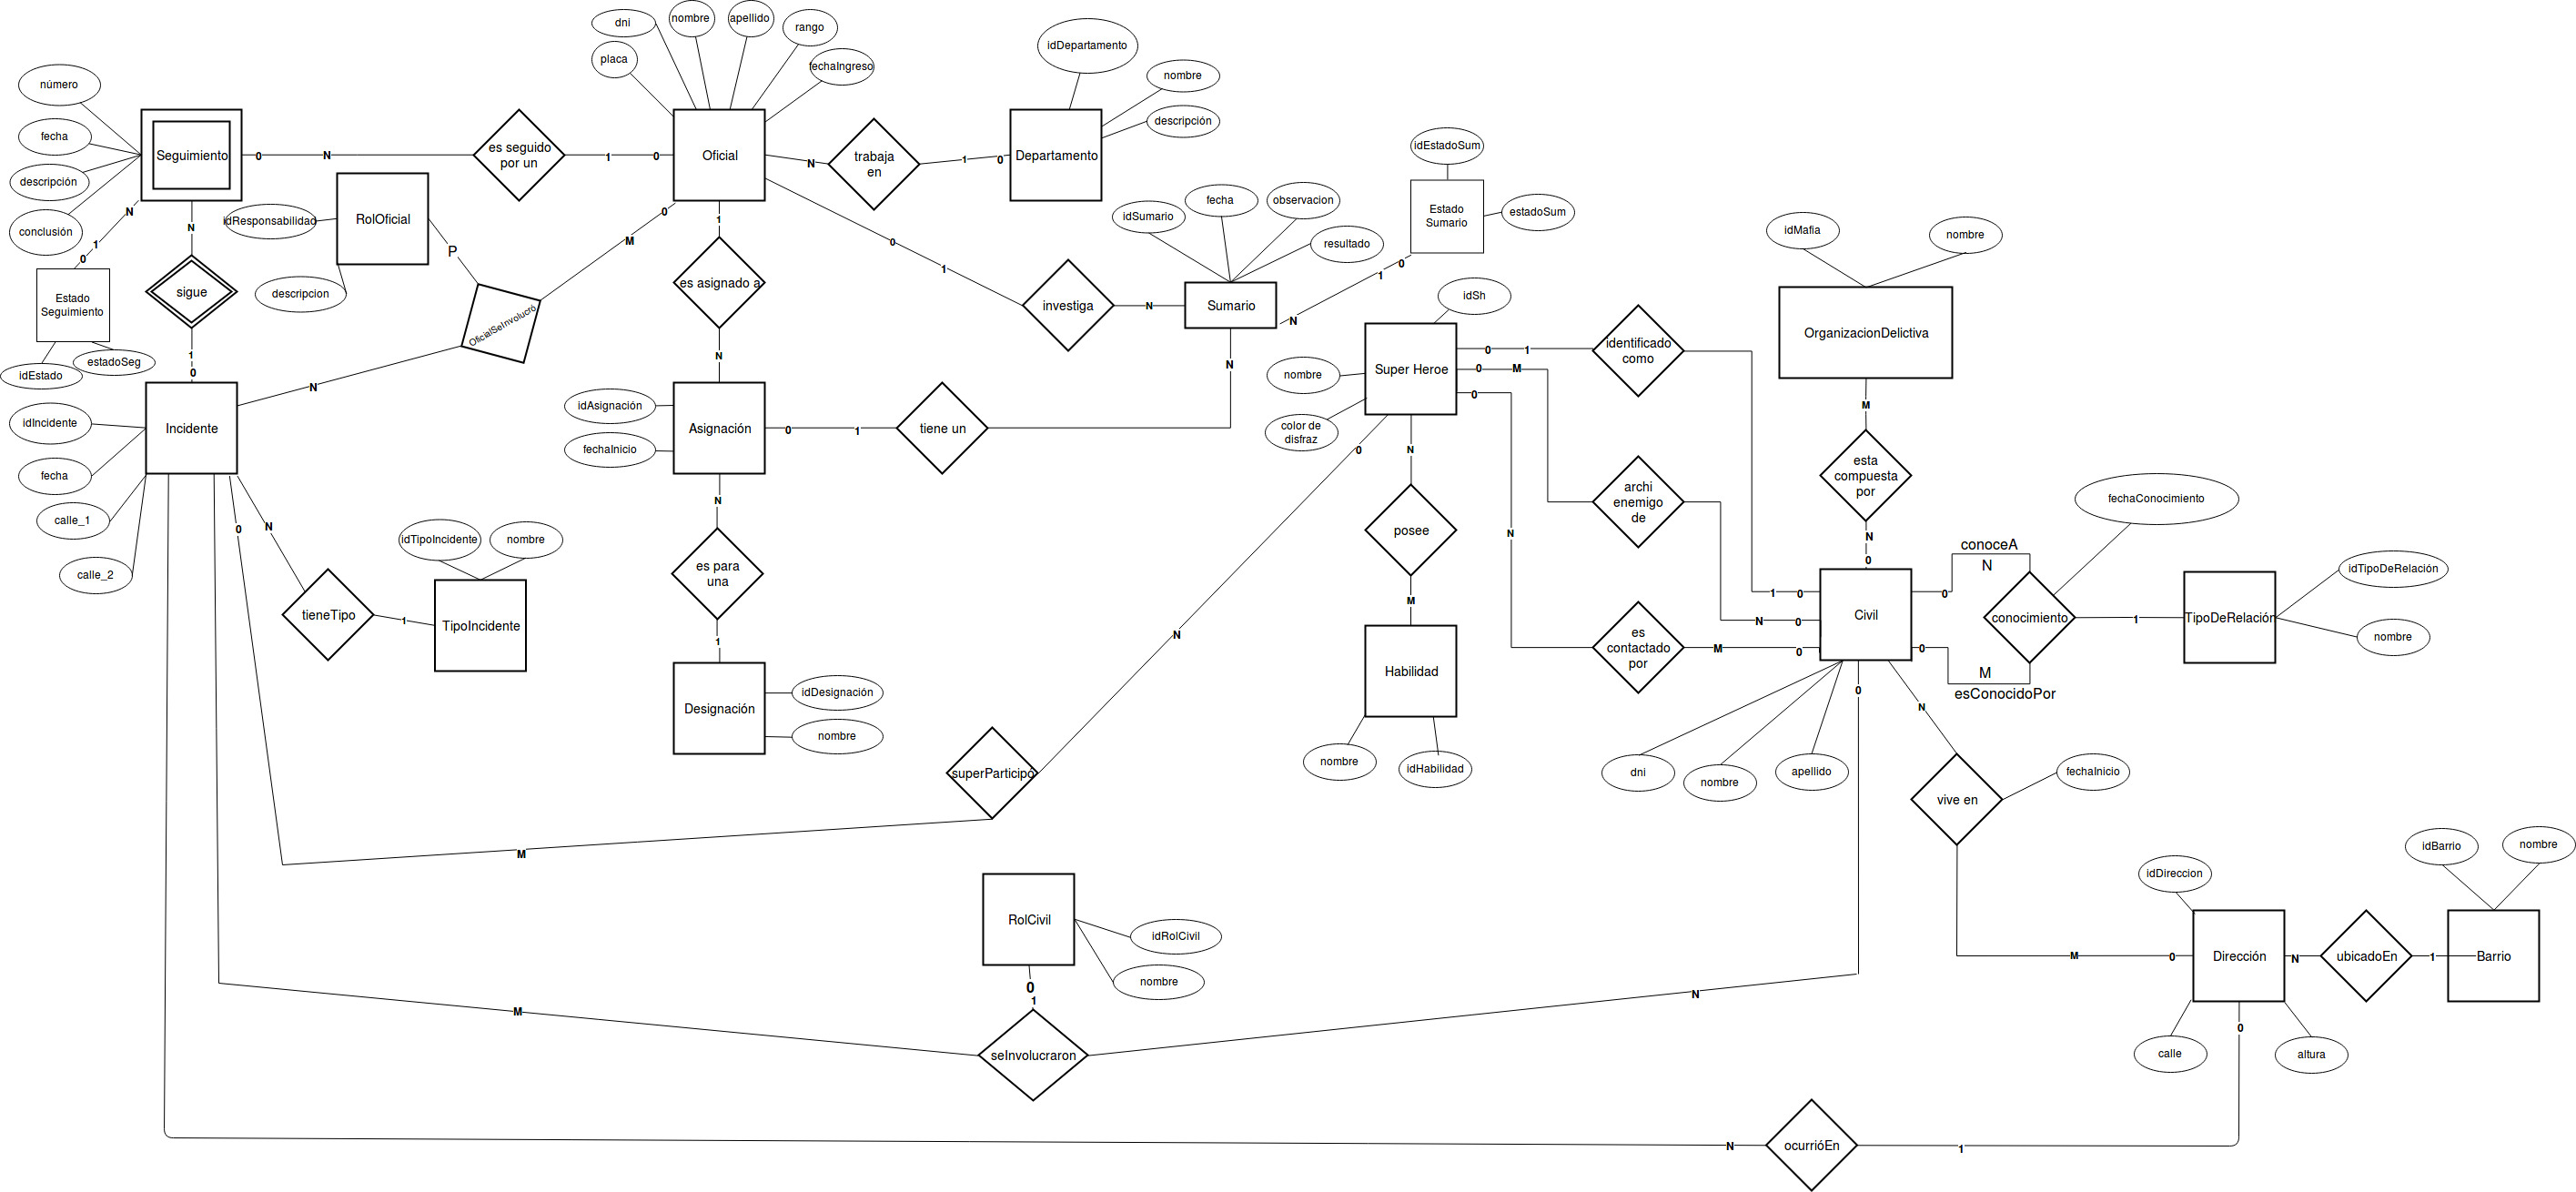
\includegraphics[scale=0.20]{MER/CiudadGotica.jpg}
  \caption{Ciudad Gótica}
  \label{fig:cg}
\end{figure}

\subsection{Modelo Relacional}\label{modelo-relacional}

\subsubsection{Entidades}\label{entidades}

Civil(\uline{dni}, nombre, apellido)\\
%PK = \{dni\}\\
%CK = \{dni\}\\

Superheroe(\uline{idSuperheroe}, nombre, color de disfraz, \dashuline{dni})\\
%PK = \{idSuperheroe\}\\
%CK = \{idSuperheroe\}\\
%FK = \{dni\}\\

Habilidad(\uline{idHabilidad}, nombre)\\

OrganizacionDelictiva(\uline{idMafia}, nombre)\\

Direccion(\uline{idDireccion}, calle, altura, \dashuline{idBarrio})\\

Barrio(\uline{idBarrio}, nombre)\\

TipoRelacion(\uline{idTipoRelacion}, nombre)\\

Incidente(\uline{idIncidente}, fecha, calle\_1, calle\_2,
\dashuline{idTipoIncidente}, \dashuline{idDireccion})\\

TipoIncidente(\uline{idTipoIncidente}, nombre)\\

Seguimiento(\uline{numero}, fecha, descripción, conclusión,
estado,\uuline{idIncidente}, \dashuline{placa}, \dashuline{idEstadoSeg})\\

EstadoSeguimiento(\uline{idEstadoSeg}, estado) \\

Departamento(\uline{idDepartamento}, nombre, descripción)\\

Oficial(\uline{placa},dni, nombre, apellido, rango, fechaIngreso, tipo,
\dashuline{idDepartamento}) \\

RolOficial(\uline{idResponsabilidad}, descripción)\\

RolCivil(\uline{idRolCivil}, nombre)\\

Asignación(\uline{idAsignación}, fechaInicio, \dashuline{idDesignación}, \dashuline{placa})\\

Sumario(\uline{idSumario}, fecha, observación, resultado, \dashuline{placa},
\dashuline{idAsignación}, \dashuline{idEstadoSum})\\

EstadoSumario(\uline{idEstadoSum}, estado) \\

Designacion(\uline{idDesignación}, nombre) \\

\subsubsection{Interrelaciones}\label{relaciones}

OficialSeInvolucró(\uuline{placa}, \uuline{idIncidente}, \uuline{idResponsabilidad})\\

Posee(\uuline{idSuperheroe}, \uuline{idHabilidad})\\

ArchienemigoDe(\uuline{idSuperheroe},\uuline{dni})\\

EsContactadoPor(\uuline{idSuperheroe},\uuline{dni})\\

SuperParticipó(\uuline{idSuperheroe}, \uuline{idIncidente})\\

EstaCompuestaPor(\uuline{idMafia}, \uuline{dni})\\

Conocimiento(\uuline{conocedor},\uuline{conocido},
fechaConocimiento, \dashuline{idTipoDeRelación})\\

seInvolucraron(\uuline{dni}, \uuline{idIncidente}, \dashuline{idRolCivil})\\

ViveEn(\uuline{dni}, \uuline{idDirección}, fechaInicio)\\

\subsubsection{Consideraciones adicionales}\label{consideraciones-adicionales}

Como en la relación \emph{identificadoComo} ambas entidades participan
parcialmente, decidimos poner la foreign key en Super Héroe, asumiendo
que esto nos generaría menos elementos nulos en la base de datos.

\subsubsection{Restricciones del modelo}

\begin{itemize}

\item\uline{\textbf{Asignación}}:
\begin{itemize}
\item Fecha de inicio mayor o igual a fecha de ingreso del oficial.
\item Asumimos que solo puede tener una asignación a una designación al mismo tiempo (misma fecha inicio). 
Cuando termina una asignación, un Oficial
empieza otra asignación en otra.
\end{itemize}


\item\uline{\textbf{Sumario:}}
\begin{itemize}
\item Fecha del sumario mayor o igual a fecha de ingreso del oficial a investigar.
\item Investigador del sumario no puede investigarse a si mismo.
\item Fecha del sumario mayor o igual a la fecha de inicio de la asignación.
\item Si el estado es concluido, entonces tiene un resultado. 
\end{itemize}
\item\uline{\textbf{Oficial:}}
\begin{itemize}
\item $dni$ únicos.
\item  Si se involucra en un incidente, la fecha de este último tiene que ser mayor o igual a la fecha de ingreso del oficial.
\end{itemize}
\item\uline{\textbf{Seguimiento:}}
\begin{itemize}
\item Solo puede ser seguida si su estado es $en$ $proceso$.
\item Si es seguida, lo es por un Oficial cuya fecha de ingreso sea menor o igual a la fecha del seguimiento.
\item Fecha del seguimiento mayor a fecha del incidente del relacionado.
\item Una vez que un proceso está en estado $cerrado$ no puede cambiar de estado y deja de estar seguido por un oficial.
\item La conclusion solo tiene un valor si el estado del seguimiento es cerrado.
\end{itemize}
\item\uline{\textbf{Rol Oficial:}}
\begin{itemize}
\item Asumimos que un oficial en un incidente puede cumplir muchos roles. Por eso es $P$ su cardinalidad en la ternaria entre esta, Oficial e Incidente de la interrelacion $OficialSeInvolucro$.
\end{itemize}

\item\uline{\textbf{Super héroe:}}
\begin{itemize}
\item No puede ser archienemigo de la misma persona de la que es $identificado$ $como$.
\item No puede ser identificado como una persona que pertence a una organizacion delictiva.
\item No puede participar como super héroe en el incidente al mismo tiempo que su correspondiente civil (si es que se conoce su identidad) se involucra como civil.
\end{itemize}
\item\uline{\textbf{Desambiguación Civil/Persona:}}
\begin{itemize}
\item  Elejimos llamar Civil a tal entidad porque entendemos que los oficiales, son personas, pero en nuestro modelo no serán Civiles. Creemos que Civil representa el aspecto cívico de un habitante de ciudad Gótica con sus propias interrelaciones y atributos.
En este modelo asumimos que no va a existir un oficial que sea civil. Por lo que estas entidades no comparten $dni$.
\item En este modelo simplificamos para que un Civil no pueda volver a vivir en una dirección.

\end{itemize}
\end{itemize}

\subsection{Consultas}

\subsubsection{Query 1}
Listado de incidentes en un rango de fechas, mostrando los datos de las personas y policías involucrados con el rol que jugó cada uno en el incidente.

\verbatiminput{Consultas/tp1-query1.txt}

\subsubsection{Query 2}
Dada una organización delictiva, el detalle de incidentes en que participaron
las personas que componen dicha organización

\verbatiminput{Consultas/tp1-query2.txt}

\subsubsection{Query 3}
La lista de todos los oficiales con sus rangos, de un departamento dado.

\verbatiminput{Consultas/tp1-query3.txt}

\subsubsection{Query 4}
El ranking de oficiales que participaron en más incidentes

\verbatiminput{Consultas/tp1-query4.txt}

\subsubsection{Query 5}
Los barrios con mayor cantidad de incidentes.

\verbatiminput{Consultas/tp1-query5.txt}

\subsubsection{Query 6}
Todos los oficiales sumariados que participaron de algún incidente.

\verbatiminput{Consultas/tp1-query6.txt}

\subsubsection{Query 7}
Las personas involucradas en incidentes ocurridos en el barrio donde viven

\verbatiminput{Consultas/tp1-query7.txt}

\subsubsection{Query 8}
Los superheroes que tienen una habilidad determinada

\verbatiminput{Consultas/tp1-query8.txt}

\subsubsection{Query 9}
Los superheroes que han participado en algún incidente.

\verbatiminput{Consultas/tp1-query9.txt}

\subsubsection{Query 10}
Listado de todos los incidentes en donde estuvieron involucrados superheroes
y fueron causados por los $archienemigos$ de los superheroes involucrados.

\verbatiminput{Consultas/tp1-query10.txt}

\subsection{Modelo Físico}

\verbatiminput{ModeloFisico/tp1Schema.txt}